\newpage
\section{Doing tropical computations}
\label{sec:tropical}
\emph{This section follows the max convention for tropical
arithmetic. For the non-constant coefficient case tropical varieties are defined as in \cite{lifting} and \cite{thesis}.}
\vspace{0.5cm}

In this section we
explain how to use Gfan to do tropical computations.  For a fixed ideal $I\subseteq
k[x_1,\dots,x_n]$ the set of all faces of all full-dimensional
Gr\"obner cones is a polyhedral complex which we call the Gr\"obner
fan of $I$. For tropical computations the lower dimensional cones of
the complex will be of our interest. In general every Gr\"obner cone
is of the form:
$$C_\omega(I):=\overline{\{\omega'\in\R^n:\init_{\omega'}(I)=\init_\omega(I)\}
}.$$ 

We define the tropical variety $\T(I)$ of an ideal $I$ to be the
the set of all $\omega$ such that $\init_\omega(I)$ does not contain a monomial.
If the ideal $I$ is homogeneous with respect to a positive grading, then the Gr\"obner cones cover all of $\R^n$ and $\T(I)$ is a union of Gr\"obner cones.
Thus for a homogeneous ideal the tropical variety gets the structure of a polyhedral fan which it inherits from the Gr\"obner fan.
%collection of all Gr\"obner cones with monomial-free initial
%ideals.
We therefore also define the tropical variety $\T(I)$ to be the collection of all Gr\"obner cones $C_\omega(I)$ such that $\init_\omega(I)$ is monomial-free.

We start by noticing that for computational purposes it is no restriction to only consider the case of a homogeneous ideal:
\begin{lemma}\cite[Lemma~6.2.5]{thesis}
\label{lem:tropical by homogenisation}
Let $I\subseteq k[x_1,\dots,x_n]$ be an ideal generated by
$f_1,\dots,f_m\in k[x_1,\dots,x_n]$. Let $J=\langle
f_1^h,\dots,f_m^h\rangle\subseteq k[x_0,\dots,x_n]$. Then $\init_\omega(I)$ is monomial-free if and
only if $\init_{(0,\omega)}(J)$ is monomial-free where $\omega\in\R^n$. In particular we have the following identity of sets in $\R^{n+1}$:
$$\{0\}\times\T(I)=\T(J)\cap(\{0\}\times\R^n).$$
\end{lemma}
Here $f^h$ denotes the homogenization of the polynomial $f$.
The homogenization of a list of polynomials can be computed by the program \texttt{gfan\_homogenize}.
Notice that the lemma only requires the generators to be homogenized as a set of polynomials and not in the sense of a polynomial ideal.

The tropical algorithms
implemented in Gfan are explained in \cite{ctv}.
% The reference also
%contains definitions and theorems needed for understanding this
%section of the manual.
Notice that Gfan follows the usual conventions
for signs of weight vectors defining initial forms while \cite{ctv}
uses opposite signs. This means that \name is compatible with the max-plus convention whereas \cite{ctv} is compatible with the min-plus convention.

\subsection{Tropical variety by brute force}
The command \texttt{gfan\_tropicalbruteforce} will compute all
Gr\"obner cones of a homogeneous ideal and for each check if its initial ideal
contains a monomial. The output is the tropical variety of the
ideal. Since the tropical variety is usually much smaller than the
Gr\"obner fan this is a rather slow method for computing the tropical
variety. The line
\begin{verbatim}
gfan_buchberger | gfan_tropicalbruteforce
\end{verbatim}
run on the input
\begin{verbatim}
Q[a,b,c,d,e,f,g,h,i,j]
{
bf-ah-ce,
bg-ai-de,
cg-aj-df,
ci-bj-dh,
fi-ej-gh
}
\end{verbatim}
produces a tropical variety of the input ideal in a few minutes as a
polyhedral fan, see Section~\ref{format:fan}. We use
\texttt{gfan\_buchberger} since \texttt{gfan\_tropicalbruteforce}
requires its input to be a marked reduced Gr\"obner basis.
\begin{remark}
Notice that if $k'\supseteq k$ is a field extension and $I\subseteq
k[x_1,\dots,x_n]$ an ideal then $\T(I)=\T(\langle
I\rangle_{k'[x_1,\dots,x_n]})$ as a polyhedral fan. This identity
follows since both objects can be computed by Gr\"obner basis methods
and Gr\"obner bases are independent of such field extensions. The same argument of course also applies to the Gr\"obner fans of the two ideals.
\end{remark}
\subsection{Traversing tropical varieties of prime ideals}
Let $I\subseteq \CC[x_1,\dots,x_n]$ be a homogeneous monomial-free
prime ideal of dimension $d$. By the Bieri Groves Theorem \cite{bg}
the tropical variety of $I$ is a pure $d$-dimensional polyhedral
fan. It is connected in codimension one (\cite[Theorem~14]{ctv}) and can be
traversed by Gfan. Let $\omega$ be a relative interior point of a
$d$-dimensional Gr\"obner cone in the tropical variety of $I$. Fix
some term order $\prec$. Gfan represents $C_\omega(I)$ by the pair of
marked reduced Gr\"obner bases
$(\G_{\prec_\omega}(\init_\omega(I)),\G_{\prec_\omega}(I))$.  To
compute the tropical variety of an ideal we must begin by finding a
starting $d$-dimensional Gr\"obner cone. For this
\texttt{gfan\_tropicalstartingcone} is used. % This programs guesses a
%starting cone by heuristic methods. The guessing might fail. In that
%case the program will terminate with an error message.
After having
computed a starting cone we use the program
\texttt{gfan\_tropicaltraverse} to traverse the tropical variety.
%There are several options for the output. In general the choice of output we request can have a huge influence on the running time for the program.
We illustrate the procedure with an example.
\begin{remark}
Gfan does its computations over $\Q$ and thus the input should be an
ideal generated by polynomials in $\Q[x_1,\dots,x_n]$. The assumption
that $I$ is an ideal in $\CC[x_1,\dots,x_n]$ is needed since by
``prime ideal'' in the above we mean ``prime ideal in the polynomial
ring over the algebraically closed field $\CC$''. If $I$ is a prime ideal in
$\Q[x_1,\dots,x_n]$ we do not know that its tropical variety is connected.
 In
Section~\ref{sec:non-constant} we address the problem of specifying non-rational
coefficients.
\end{remark}
\begin{example}
Let $I\subseteq\Q[a,\dots,o]$ be the ideal generated by the relations
on the 2 by 2 minors of a 2 by 6 generic matrix.  In $\CC[x_1,\dots,x_n]$ the
ideal $I$ generates a prime ideal.  To get a starting cone for the
traversal of $\T(I)$ we run the command
\begin{verbatim}
gfan_tropicalstartingcone
\end{verbatim}
on the input
\begin{verbatim}
Q[a,b,c,d,e,f,g,h,i,j,k,l,m,n,o]
{
bg-aj-cf,  bh-ak-df,  bi-al-ef,  ck-bm-dj,  ch-am-dg,
cl-ej-bn,  ci-eg-an,  dn-co-em,  dl-bo-ek,  di-ao-eh,
gk-fm-jh,  gl-fn-ij,  hl-fo-ik,  kn-jo-lm,  hn-im-go
}
\end{verbatim}
and get a pair of marked reduced Gr\"obner bases
\begin{verbatim}
Q[a,b,c,d,e,f,g,h,i,j,k,l,m,n,o]
{
l*m+j*o,  i*m+g*o,  i*k-h*l,  i*j-g*l,  h*j-g*k,
e*m+c*o,  e*k+b*o,  e*j-c*l,  e*h+a*o,  e*g-c*i,
c*k-b*m,  c*h-a*m,  b*i-a*l,  b*h-a*k,  b*g-a*j}
{
l*m-k*n+j*o, i*m-h*n+g*o, i*k-h*l+f*o, i*j-g*l+f*n, h*j-g*k+f*m,
e*m-d*n+c*o, e*k-d*l+b*o, e*j-c*l+b*n, e*h-d*i+a*o, e*g-c*i+a*n,
c*k-d*j-b*m, c*h-d*g-a*m, b*i-e*f-a*l, b*h-d*f-a*k, b*g-c*f-a*j}
\end{verbatim}
This takes about a second. We store the output in the file \texttt{grassmann2\_6.cone} for later use. Since $I$ has many symmetries we add the following lines describing the symmetry group to the end of the file:
\begin{verbatim}
{
(0,8,7,6,5,4,3,2,1,14,13,11,12,10,9),
(5,6,7,8,0,9,10,11,1,12,13,2,14,3,4)
}
\end{verbatim}
We are ready to traverse $\T(I)$.
% We start by running the program with the simplest possible output and using symmetries:
We run the following command
\begin{verbatim}
gfan_tropicaltraverse --symmetry <grassmann2_6.cone
\end{verbatim}
The computation takes a few (two - three) minutes. The output looks like this:
\begin{verbatim}
_application PolyhedralFan
_version 2.2
_type PolyhedralFan

AMBIENT_DIM
15

DIM
9

LINEALITY_DIM
6

RAYS
0 0 -1 0 0 0 0 0 0 0 0 0 0 0 0	# 0
0 0 0 0 0 0 0 -1 0 0 0 0 0 0 0	# 1
0 0 0 0 0 0 0 0 0 0 0 -1 0 0 0	# 2
0 0 0 -1 0 0 0 0 0 0 0 0 0 0 0	# 3
0 0 0 0 0 0 -1 0 0 0 0 0 0 0 0	# 4
0 -1 0 0 0 0 0 0 0 0 0 0 0 0 0	# 5
0 0 0 0 0 0 0 0 -1 0 0 0 0 0 0	# 6
0 0 0 0 0 0 0 0 0 0 -1 0 0 0 0	# 7
0 0 0 0 0 0 0 0 0 0 0 0 0 -1 0	# 8
0 0 0 0 0 -1 0 0 0 0 0 0 0 0 0	# 9
0 0 0 0 -1 0 0 0 0 0 0 0 0 0 0	# 10
0 0 0 0 0 0 0 0 0 0 0 0 0 0 -1	# 11
0 0 0 0 0 0 0 0 0 -1 0 0 0 0 0	# 12
-1 0 0 0 0 0 0 0 0 0 0 0 0 0 0	# 13
0 0 0 0 0 0 0 0 0 0 0 0 -1 0 0	# 14
0 0 0 -1 -1 -1 -1 0 0 -1 0 0 0 0 -1	# 15
-1 -1 0 0 0 -1 0 0 0 0 0 0 -1 -1 -1	# 16
-1 0 0 0 -1 0 0 0 -1 -1 -1 0 -1 0 0	# 17
1 1 0 0 0 1 2 2 0 2 2 0 1 1 1	# 18
1 0 2 2 1 0 0 0 1 1 1 0 1 2 2	# 19
0 0 0 1 1 1 1 0 0 1 2 2 2 2 1	# 20
1 1 0 2 2 1 0 2 2 0 0 0 1 1 1	# 21
1 2 2 0 1 2 2 0 1 1 1 0 1 0 0	# 22
2 2 0 1 1 1 1 0 2 1 0 2 0 0 1	# 23
0 -1 0 -1 0 0 -1 0 -1 0 -1 0 0 -1 0	# 24

N_RAYS
25

LINEALITY_SPACE
0 0 0 0 0 1 1 1 1 1 1 1 1 1 1
0 0 0 0 1 0 0 0 1 0 0 1 0 1 1
0 0 0 1 0 0 0 1 0 0 1 0 1 0 1
0 0 1 0 0 0 1 0 0 1 0 0 1 1 0
0 1 0 0 0 0 -1 -1 -1 0 0 0 -1 -1 -1
1 0 0 0 0 0 0 0 0 -1 -1 -1 -1 -1 -1

ORTH_LINEALITY_SPACE
0 0 0 0 0 0 0 0 0 0 1 -1 -1 1 0
0 0 0 0 0 0 0 0 0 1 0 -1 -1 0 1
0 0 0 0 0 0 0 1 -1 0 0 0 -1 1 0
0 0 0 0 0 0 1 0 -1 0 0 0 -1 0 1
0 0 0 0 0 1 0 0 -1 0 0 -1 -1 1 1
0 0 0 1 -1 0 0 0 0 0 0 0 -1 1 0
0 0 1 0 -1 0 0 0 0 0 0 0 -1 0 1
0 1 0 0 -1 0 0 0 0 0 0 -1 -1 1 1
1 0 0 0 -1 0 0 0 -1 0 0 0 -1 1 1

F_VECTOR
1 25 105 105
\end{verbatim}
After this follows a list of cones and maximal cones.
Every maximal cone has an associated multiplicity which is also listed.

The output says that the tropical variety has dimension $9$. Modulo the
$6$-dimensional homogeneity space this is reduced to a $3$-dimensional complex in
$\R^9$ and thus we may think of the tropical variety as a
$2$-dimensional polyhedral complex on the $8$-sphere in $\R^9$. This
complex is simplicial and has $105$ maximal cones.


The extreme rays (modulo the homogeneity space) are labeled
$0,\dots,24$. In the cone lists the cones are grouped together
according to dimension and orbit with respect to the specified
symmetries. See Section~\ref{sec:format fan} for more information on how to read the
polyhedral fan format.
\end{example}

%If we look carefully in the debug output from the program we
%will also see that these $105$ cones come in $17$ orbits.  If we
%wanted to know more about the traversed cones we could use the option
%\texttt{--largedimensional}. This will list the $d$-dimensional and
%$(d-1)$-dimensional cones of the fan. In our example one of the
%$d$-dimensional cones is listed like this: (In this manual lines have
%been concatenated to avoid wasting paper)

While traversing the variety the program
\texttt{gfan\_tropicaltraverse} only computes $d$ and
$(d-1)$-dimensional cones. The other cones are extracted after
traversing. Also the symmetries are expanded. Sometimes extracting all
cones is time consuming and one is only interested in the high
dimensional cones up to symmetry. These can be output using the option
\texttt{--noincidence}. In that case the output would be a list of
orbits for maximal cones and a list of orbits for codimension one
cones. It is also listed how these cones are connected taking symmetry
into account. In general that format is rather difficult to read.


A final remark about \texttt{gfan\_tropicaltraverse} is that the
polyhedral structure of the complex comes from the Gr\"obner fan. For
some ideals it is possible to find polyhedral fans covering the
tropical variety with fewer cones.


\subsection{Intersecting tropical hypersurfaces (partially deprecated)}
{\bf Note: While the content of this subsection is still correct, the command \texttt{gfan\_tropicalprevariety}, new in gfan0.7 and presented in Section~\ref{subsec:tropicalprevariety}, is generally much faster than \texttt{gfan\_tropicalintersection}. The old functionality is kept for compatability - in particular regarding grouping of its output and handling of symmetry and stable intersections.}

The tropical variety of a principal ideal is called a \emph{tropical
hypersurface}. A \emph{tropical prevariety} is a finite intersection of
tropical hypersurfaces or, to be precise, the intersection of the
support set of these hypersurfaces. In Gfan the intersection is
represented by the \emph{common refinement} of the tropical
hypersurfaces. The program \texttt{gfan\_tropicalintersection} can
compute such intersections.
\begin{example}
To compute the intersection of the tropical hypersurfaces $\T(\langle a+b+c+1\rangle)$ and $\T(\langle a+b+2c\rangle)$ we run
\begin{verbatim}
gfan_tropicalintersection
\end{verbatim} 
on
\begin{verbatim}
Q[a,b,c]
{a+b+c+1,a+b+2c}
\end{verbatim}
The output is a polyhedral fan whose support is the intersection. The
balancing condition for this fan is not satisfied which implies that it
is not a tropical variety.
%list of cones whose union is the tropical prevariety.  Notice, as a polyhedral complex, some cones might be missing from the list but all maximal cones are present. The program also gives a list with a relative interior point for each cone. 

%If we use the option \texttt{--incidence} we will get more information about the combinatorial structure of the intersection as a polyhedral complex. We should note that this option only investigates the maximal dimensional complex.

%An interesting question is if the intersection equals the tropical variety of the ideal generated by the input polynomials. A necessary condition for this to be true is that all the computed relative interior points pick out monomial-free initial ideal. This can be checked with the option \texttt{-t}. In our example the prevariety is not equal to the tropical variety and the program will find a vector that proves this.
\end{example}

\subsection{Computing tropical bases of curves}
In Gfan an ideal $I$ is said to define a \emph{tropical curve} if
$k[\x_1,\dots,x_n]/I$ has Krull dimension equal to or one larger than the
dimension of the homogeneity space of $I$.  A \emph{tropical basis} of $I$ is
a finite generating set for the ideal such that the tropical variety
defined by $I$ (as a set) is the intersection of the tropical
hypersurfaces of the generators. A tropical basis always exists \cite{ctv}.  The
program \textup{gfan\_tropicalbasis} computes a tropical basis for an
ideal defining a tropical curve.
\begin{example}
Again we consider the ideal $\langle a+b+c+1,a+b+2c\rangle$. We notice that this ideal defines a curve since the Krull dimension is $1$ and the dimension of the homogeneity space is $0$. In the example above we saw that the listed set is not a tropical basis. We run
\begin{verbatim}
gfan_tropicalbasis -h
\end{verbatim}
on
\begin{verbatim}
Q[a,b,c]
{a+b+c+1,a+b+2c}
\end{verbatim}
to get some tropical basis
\begin{verbatim}
Q[a,b,c]
{
-1+c,
2+b+a}
\end{verbatim}
We needed the option \texttt{-h} here since the ideal was not homogeneous. If we run \texttt{gfan\_tropicalintersection} on the output we see that the tropical variety consists of three rays and the origin.
\end{example}


\subsection{Tropical intersection theory}
Gfan contains a few experimental programs for doing computations in
tropical intersection theory. In \cite[Definition 3.4]{allermannRau}
the tropical Weil divisor of a tropical rational function on a
(tropical) $k$-cycle in $\R^n$ is defined. This divisor can be
computed in Gfan. However, Gfan and \cite{allermannRau} do not agree
on the basic definitions in tropical geometry. For example the
definition of a fan is different. Here we will adjust the necessary
definitions to the Gfan conventions. A tropical $k$-cycle will be a
pure (rational) polyhedral fan $F$ of dimension $k$ in $\R^n$ with
weights which is balanced in the following sense: To every
$k$-dimensional facet $C$ we assign a weight (or multiplicity)
$m_C\in\Z$. The vector space $\R^n$ comes with its standard lattice
$\Z^n$. For a $k-1$-dimensional ridge $R\in F$ and a facet $C$ in its
star\footnote{the smallest polyhedral subcomplex of $F$ containing all
faces of $F$ containing $R$.} in $F$ corresponding to a cone $L$ in
the link\footnote{take an $\epsilon$-ball around a relative interior
$\omega\in R$ and intersect it with $F$. Translating the ball to the
origin and scaling the intersection to infinity we get the link of $R$
in $F$.} of $R$ in $F$, the semi-group
$L\cap\Z^n/\textup{span}_{\R}(R)\cap\Z^n\subseteq
\Z^n/\textup{span}_{\R}(R)\cap\Z^n$ is isomorphic to $\N$. Define
$u_{C/R}\in \Z^n/\textup{span}(R)\cap\Z^n$ as the element identified
with $1\in\N$. The balancing condition at $R$ is that
$$\sum_{C\in F:R\subset C} m_Cu_{C/R}=0.$$
For a (weighted) fan to be a tropical cycle this must hold at every ridge $R$.

It remains to define what a tropical rational function is. Take a
polyhedral fan $F'$ and associate to each of its maximal cones a
linear form. When evaluating a point $x$ in the support of $F'$ simply
evaluate the linear form of cone containing $x$. If this gives a
well-defined function we call this function a tropical rational
function.  When computing Weil divisors we will require that the supports satisfy
$\textup{supp}(F)\subseteq \textup{supp}(F')$.  There will be no further restriction
on the polyhedral structure.

For a definition of the Weil divisor itself we refer
to \cite[Definition 3.4]{allermannRau}. Here we just mention that it
again is a cycle of dimension one lower.

To demonstrate the Gfan features we recompute \cite[Example 3.10]{allermannRau}.
An easy way to generate the $k$-cycle of that example is to compute it as a hypersurface. Since the paper is using min and Gfan is using max we need to change the polynomial from the paper such that the Newton polytope is flipped:
\begin{verbatim}
gfan_tropicalhypersurface > tmpfile1.poly
Q[x_1,x_2,x_3]
{x_2x_3+x_1x_3+x_1x_2+x_1x_2x_3}
\end{verbatim}
The weights/multiplicities are stored in the MULTIPLICITIES section of the Polymake file.

It is harder specifying the rational function. We make the following file and call in \texttt{func.poly}.
\begin{footnotesize}
\begin{verbatim}
_application PolyhedralFan
_version 2.2
_type PolyhedralFan

AMBIENT_DIM
3

DIM
2

LINEALITY_DIM
0

RAYS
1 0 0	# 0
0 1 0	# 1
0 0 1	# 2
-1 -1 -1	# 3
1 1 0	# 4
-1 -1 0	# 5

N_RAYS
6

LINEALITY_SPACE

ORTH_LINEALITY_SPACE
1 0 0
0 1 0
0 0 1

MAXIMAL_CONES
{3 5}	# Dimension 2
{5 2}
{0 2}
{1 2}
{1 3}
{0 3}
{1 4}
{0 4}

MULTIPLICITIES
1
1
1
1
1
1
1
1

RAY_VALUES
0
0
0
1
-1
0

LINEALITY_VALUES
\end{verbatim}
\end{footnotesize}
Instead of specifying the linear function on each maximal cone we have
to specify its values on each of the rays in the fan and each of the
generators of the lineality space. Then Gfan will automatically
interpolate the function. Since the lineality space of the fan is
empty we leave the LINEALITY\_VALUES section empty.

We now compute the Weil divisor:
\begin{footnotesize}
\begin{verbatim}
gfan_tropicalweildivisor -i1 tmpfile1.poly -i2 func.poly >tmpfile2.poly
\end{verbatim}
\end{footnotesize}
...and compute the Weil divisor again as in \cite{allermannRau}...
\begin{footnotesize}
\begin{verbatim}
gfan_tropicalweildivisor -i1 tmpfile2.poly -i2 func.poly >tmpfile3.poly
\end{verbatim}
\end{footnotesize}
We get a fan with the origin being the only cone. It has multiplicity $-1$:
\begin{verbatim}
MULTIPLICITIES
-1      # Dimension 0
\end{verbatim}

There is another useful command for computing polyhedral fans for
rational functions. The command \texttt{gfan\_tropicalfunction} takes a
polynomial and turns it into a fan representing its tropicalization
which is a tropical rational function.

\subsection{Non-constant coefficients (partially deprecated)}
\label{sec:non-constant}
{\bf The easiest way to compute tropical prevarieties is by using the command {\texttt gfan\_tropicalprevariety} introduced in gfan0.7. See Section~\ref{subsec:tropicalprevariety}. The current section is kept for compatibility reasons.}

In tropical geometry it is common to take the valuation of
$\CC\{\{t\}\}$ into account when defining the tropical variety of
an ideal in $\CC\{\{t\}\}[x_1,\dots,x_n]$.  Here $\CC\{\{t\}\}$ denotes the field of
Puiseux series. The valuation $\textup{val}(p)$ of a non-zero Puiseux
series $p$ is the degree of its lowest order term.


\begin{definition}
\label{def:tomegadegree}
For $\omega\in\R^n$ the \emph{t-$\omega$-degree}\index{t-$\omega$-degree} of a term $ct^ax^v$
with $c\in\CC^*$, $a\in \Q$ and $v\in\Z^n$ is defined as
$-\val(ct^a)+\omega\cdot v=-a+\omega\cdot v$.  The \emph{t-initial
form}\index{t-initial form} $\tinit_\omega(f)\in\CC[x_1,\dots,x_n]$ of a polynomial
$f\in\puiseux[x_1,\dots,x_n]$ is the sum of all terms in $f$ of maximal
t-$\omega$-weight but with $1$ substituted for $t$.
\end{definition}
\begin{remark}
Notice that since $t$ has t-$\omega$-degree $-1$, the maximal
t-$\omega$-weight \emph{is} attained by a term if the polynomial is
non-zero. Furthermore, only a finite number of terms attain the
maximum. Therefore, it makes sense to substitute $t=1$ and consider
the finite sum of terms as a polynomial in $\CC[x_1,\dots,x_n]$.
\end{remark}
\begin{example}
Consider $f=(1+t)+t^2x+tx^2\in\puiseux[x_1,\dots,x_n]$. Let $\omega=({1\over
2})\in\R^1$. Then $\tinit_\omega(f)=1+x^2$. For any
other choice of $\omega$ the t-initial form is a monomial.
\end{example}
\begin{definition}
Let $I\subseteq \puiseux[x_1,\dots,x_n]$ and $\omega\in\R^n$. The \emph{t-initial ideal}\index{t-initial ideal} of $I$ with respect to $\omega$ is defined as:
$$\tinit_\omega(I):=\langle \tinit_\omega(f):f\in I\rangle\subseteq\CC[x_1,\dots,x_n].$$
\end{definition}

\begin{definition}
\label{def:tropvar}
Let $I\subseteq \puiseux[x_1,\dots,x_n]$ be an ideal. The \emph{tropical variety} of $I$ is the set
$$\T'(I):=\{\omega\in\R^n:\tinit_\omega(I) \textup{ is monomial-free}\}.$$
%Here monomial-free\index{monomial-free} means that the ideal does not contain a monomial.
\end{definition}
We use the notation $\T'(I)$ to avoid contradicting our original definition
of the tropical variety of an ideal in the polynomial ring over a
field.
%An important theorem says that the tropical variety of $I$ is also the
%negative of the closure of the image of $V(I)\subseteq \CC\{\{t\}\}^*$
%under the coordinatewise valuation.


\begin{proposition} \cite[Proposition~7.3]{lifting}
\label{prop:computing tinit}
Let $I\subseteq \CC[t,x_1,\dots,x_n]$ be an ideal, $J=\langle I\rangle_{\puiseux[x_1,\dots,x_n]}$ and $\omega\in\R^n$. Then $\textup{t-in}_\omega(I)=\textup{t-in}_\omega(J)$.
\end{proposition}

\begin{remark}
\label{rem:computing tinit}
For $f\in\CC[t,x_1,\dots,x_n]$ we have
$\tinit_\omega(f)=(\init_{(-1,\omega)}(f))|_{t=1}$. Consequently, for
$I\subseteq\CC[t,x_1,\dots,x_n]$ we have
$\tinit_\omega(I)=(\init_{(-1,\omega)}(I))|_{t=1}$. In order to
decide if $\tinit_\omega(I)$ contains a monomial we may simply decide if the initial ideal
$\init_{(-1,\omega)}(I)$ contains a monomial.
 As a corollary we get
$$\T(I)\cap(\{-1\}\times\R^n)=\{-1\}\times\T'(J).$$

In fact this gives a method for computing the tropical variety as a set of any
ideal $J\subseteq\CC\{\{t\}\}[x_1,\dots,x_n]$ generated by elements
in the polynomial ring over the field of rational functions
$\Q(t)[x_1,\dots,x_n]$ in Gfan by clearing denominators and
intersecting the result with the $t=-1$ plane.  (We remind the reader
that Lemma~\ref{lem:tropical by homogenisation} shows that for
computational purposes it is no restriction if $I$ is not
homogeneous.)
\end{remark}

Intersecting the tropical variety with the $t=-1$ plane can with some difficulty be done by
hand. If the tropical (pre)-variety has been computed with
\texttt{gfan\_tropicalintersection} then it is also possible to let Gfan do
the intersection. What Gfan does is to compute the common refinement
of the fan with the fan consisting of the halfspace $t\leq 0$ and its
proper face. Of course this does not remove the cones in the $t=0$
plane, but they are easily removed by hand. We illustrate the
procedure by an example.

\begin{example}
\label{ex:nonconstant}
Exercise 2 in Chapter 9 of \cite{sturmfelssolving} asks us to draw the variety
defined by the \emph{tropical} polynomial
$f=1x^2+2xy+1y^2+3x+3y+1$. If we tropically divide this polynomial by $3$ we get $f':=f/3=-2x^2-1xy-2y^2+0x+0y+-2$ which defines the same tropical variety. This variety equals the variety defined by
the polynomial $g=t^2x^2+txy+t^2y^2+x+y+t^2\in\CC\{\{t\}\}[x,y]$. Notice that $f'$ is the tropicalisation of $g$.

According to Remark~\ref{rem:computing tinit} above the we may compute $\T'(\langle g\rangle)$ by computing
the variety of $\langle t^2x^2+txy+t^2y^2+x+y+t^2\rangle\subseteq \CC[t,x,y]$ and intersecting it with the hyperplane $t=-1$.
Running
\begin{verbatim}
gfan_tropicalintersection --tplane
\end{verbatim}
on
\begin{verbatim}
Q[t,x,y]
{t^2x^2+txy+t^2y^2+x+y+t^2}
\end{verbatim}
we get
\begin{verbatim}
RAYS
0 -1 0	# 0
-1 2 1	# 1
0 1 1	# 2
-1 1 1	# 3
-1 -2 -2	# 4
0 0 -1	# 5
-1 1 2	# 6

MAXIMAL_CONES
{3 4}	# Dimension 2
{2 6}
{1 3}
{1 2}
{3 6}
{4 5}
{0 4}
{0 6}
{1 5}
\end{verbatim}
among other information. We can now draw the two-dimensional picture
asked for in the exercise.  The rays with non-zero first coordinate
become points in the picture. (If the first coordinate is not $-1$ scaling
is required to get the rational $x,y$-coordinates.) The rays with zero
first coordinate become directions. The maximal cones show how to
connect the rays; see Figure~\ref{fig:nonconstant}. Notice that some
of the connections could have been ``at infinity''.
\begin{figure}
\begin{center}
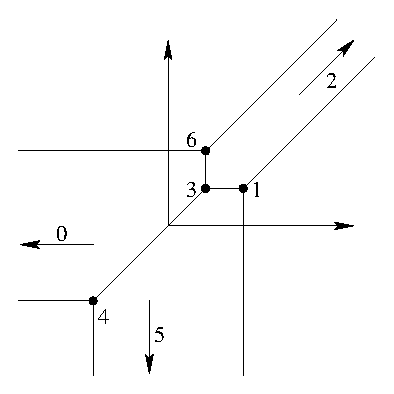
\epsfig{file=nonconst.eps,height=5.5cm} 
\end{center}
\caption{The tropical variety defined by the tropical polynomial in Example~\ref{ex:nonconstant}.}
\label{fig:nonconstant}
\end{figure}

\end{example}

\subsubsection{Algebraic field extensions of $\Q$}
Ignoring time, memory usage and overflows Gfan can compute the tropical variety $\T'(I)$ of any ideal $I\subseteq \puiseux[x_1,\dots,x_n]$ generated by elements of $\overline{\Q}(t)[x_1,\dots,x_n]$. This is a consequence of the following lemma:
\begin{lemma}\cite[Lemma~3.12]{lifting}
\label{lem:fieldextension}
Let $k$ be a field and $M=\langle m\rangle\subseteq k[a]$ a maximal ideal where $m$ is not a monomial. Let 
$I\subseteq (k[a]/M)[x_1,\dots,x_n]$ be an ideal. For $\omega\in\R^n$ we
have
$$\init_\omega(I) \textup{ contains a monomial} \Longleftrightarrow \init_{(0,\omega)}(\varphi^{-1}(I)) \textup{ contains a monomial}$$ 
where $\varphi:k[a,x_1,\dots,x_n]\rightarrow (k[a]/M)[x_1,\dots,x_n]$ is the homomorphism taking elements to their cosets.
\end{lemma}

\subsection{Tropical prevarieties}
\label{subsec:tropicalprevariety}
As explained earlier, a tropical prevariety is defined to be an intersection of finitely many tropical hypersurfaces. Such intersection can be computed by either the old command {gfan\_tropicalintersection} or the new command {gfan\_tropicalprevariety} introduced in \name version 0.7.

There are several choices to be made when defining the tropical prevariety of a list of polynomials in $\puiseux[x_1,\dots,x_n]$, for example whether $t$ should have valuation $+1$ or $-1$, whether the value group should be ordered in the positive or negativ direction (and whether gfan should ``cone over'' the complex at $x_0=-1$ or $x_0=1$ to get the fan-like output).

However, the most sensible choices are just to have the equation $$T(I)\cap\Q^n=\textup{val}(V(I))$$ satisfied, where $\textup{val}$ is cooridinate-wise valuation. This leaves the choice of thinking of $\puiseux$ as having increasing exponents in $t$ (min) or decreasing exponents in $t$ (max) and taking valuation to be $t$-exponent of the leading term of a series. 

In addition to these choices, part of the literature mixes max and min conventions to have increasing Puiseux series while following conventions of the (global) Gr\"obner fan theory (using \emph{outer} normals). This is consistent with Definition~\ref{def:tomegadegree}.
For these choices the following equation holds:
$$T(I)\cap\Q^n=-\textup{val}(V(I)).$$

In the following we illustrate these choices on some examples. Note that the \name parser only understands ordinary polynomials at the moment. So although we can specify the coefficient field to be rational functions in $t$, only polynomial of $\CC(t)[x_1,\dots,x_n]\subset\puiseux[x_1,\dots,x_n]$ that are actually in $\CC[t,x_1,\dots,x_n]$ can be parsed at the moment, leading to some inconvenience. Moreover, specifying for example $p$-adic valuations for ideals in $\Q[x_1,\dots,x_n]$ is not possible at the moment.

The command {gfan\_tropicalprevariety} has two options to set max/min conventions:
\begin{verbatim}
--mint
--minx
\end{verbatim}

\begin{example}[Default: Max, max]
The Puiseux series are decreasing in $t$-exponent and $T(I)\cap\Q^n=\textup{val}(V(I))$ is satisfied. This convention is compatible with most of \name, but seems to not be used much in the literature. One place it is used is in the introduction of~\cite{ctv}. In the following note that it would not be possible for \name to parse \texttt{(t4+1)x} while \texttt{t4x+1x} can be parsed.

\begin{verbatim}
gfan _tropicalprevariety --usevaluation
Q(t)[x]{t+t4x+1x+tx3}
\end{verbatim}
gives as part of the output
\begin{verbatim}
RAYS
1 -3	# 0
2 3	# 1
\end{verbatim}
The tropical prevariety is $\{-3,{3\over 2}\}$.
%Here the convention is that Puiseux series are increasing in $t$-exponent.
%For example taking $(i+higher order terms,0+higher order terms)$ makes equations vanish in $t$-degree 1, when substituting in.
\end{example}


\begin{example}[Max convention, increasing t-exponents]
We now change to the definition that is compatible both with the Gr\"obner basis convention (outer normals) and increasing t-exponents. This convention was used in~\cite{sturmfelssolving}, \cite{lifting} and~\cite{thesis} and satisfies $T(I)\cap\Q^n=-\textup{val}(V(I))$.
\begin{verbatim}
gfan _tropicalprevariety --usevaluation --mint
Q(t)[x]{t+t4x+1x+tx3}
\end{verbatim}
gives as part of the output
\begin{verbatim}
RAYS
1 -1	# 0
2 1	# 1
\end{verbatim}
%Here the convention is that Puiseux series are increasing in $t$-exponent.
%The rays appear in different order. Notice also the change of sign in the $t$-coordinate.
The tropical prevariety is $\{-1,{1\over 2}\}$.
\end{example}

\begin{example}[Min convention, increasing t-exponents]
Our final example illustrates the most common convention, since this is the one used in the tropical book by Maclagan and Sturmfels~\cite{tropicalbook}. It was also used in~\cite{tropgrass}. The convention has the advantage that Puiseux series are increasing in $t$ and the equation $T(I)\cap\Q^n=\textup{val}(V(I))$ is satisfied.
\begin{verbatim}
gfan _tropicalprevariety --usevaluation --mint --minx
Q(t)[x]{t+t4x+1x+tx3}
\end{verbatim}
gives as part of the output
\begin{verbatim}
RAYS
1 1	# 0
2 -1	# 1
\end{verbatim}
The tropical prevariety is $\{1,-{1\over 2}\}$.
\end{example}
More interesting examples are obtained by introducing more variables and polynomials, but here we only wished to demonstrate various conventions.

To speed up computation the arithmetic can be changed to machine-integer using for example option \texttt{--bits64}. Note that in that case overflow checking is not completely implemented.

If \texttt{--usevaluation} is not specified, then the output lives in a space of dimension one lower. If a coefficient field without a default valuation is specified in the input, then the trivial valuation is used.
